\documentclass[10pt]{article}
\usepackage[top=3cm, bottom=3cm, left=3cm, right=3cm]{geometry}

\usepackage{amsmath}
\usepackage{amssymb}
\usepackage{amsthm}
\usepackage[center]{caption}
\usepackage{comment}
\usepackage{listings}
\usepackage{multicol}
\usepackage{float}
\usepackage{mdframed}
\usepackage{hyperref}
\usepackage{pdfpages}
\usepackage{graphicx}
\usepackage{rotating}
\usepackage{tabularray}
\usepackage{framed}

\newcommand{\hrefblue}[3][blue]{\href{#2}{\color{#1}{#3}}}%

\title{Z23 Manual}
\author{Devin Singh \\ \hrefblue{mailto:singh956@purdue.edu}{singh956@purdue.edu}}

\begin{document}

\maketitle

\begin{figure}[!b]
	\begin{center}
		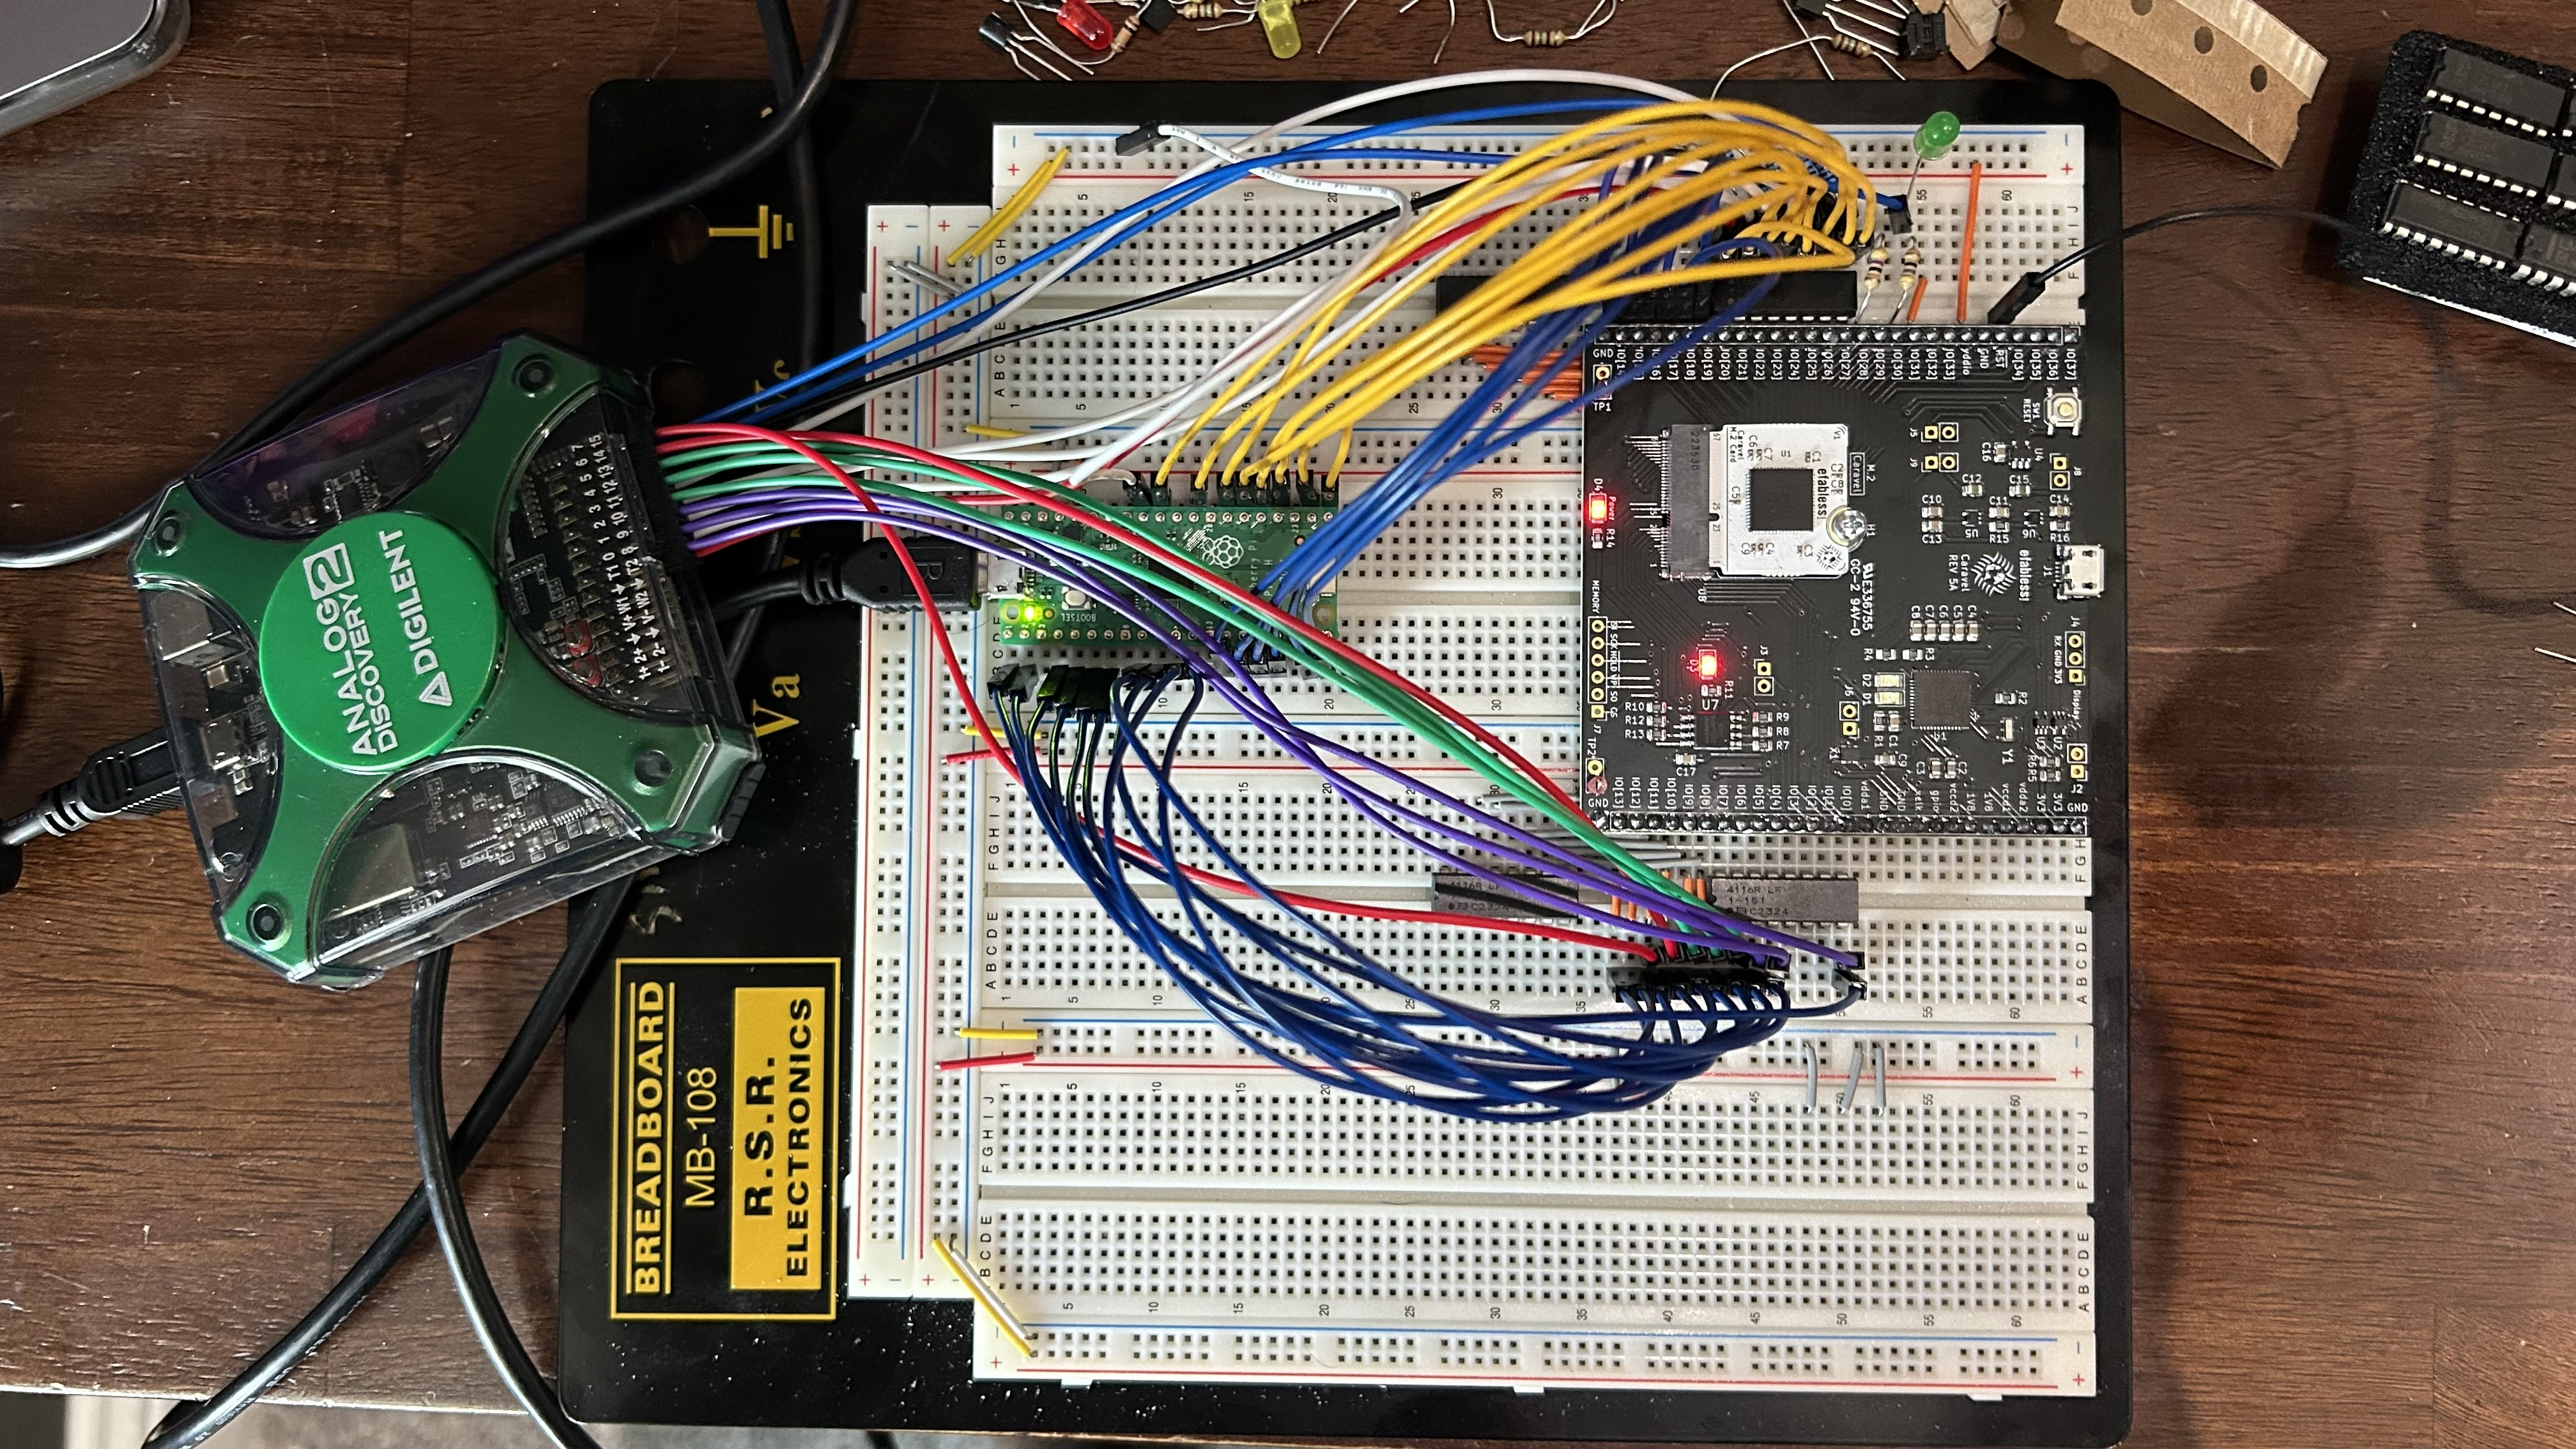
\includegraphics[width=\textwidth]{built.jpeg}
	\end{center}
\end{figure}

\newpage

\section{Z23}

The Z23 is an accumulator based, 8-bit CPU based off the
\hrefblue{https://en.wikipedia.org/wiki/Zilog_Z80}{Zilog Z80} developed during Summer 2023 as part of
the \hrefblue{https://engineering.purdue.edu/semiconductors/stars}{Purdue STARS Program}. It supports
most of the instructions of the Z80 except those using the shadow registers. An instruction table
can be seen in Figure \ref{fig:instruction_set}. More information on the effects of each instruction
can be found at \hrefblue{http://z80-heaven.wikidot.com/opcode-reference-chart}{this reference guide}.
The CPU has eight 8-bit registers which can be used in pairs to perform 16-bit memory accesses.
There are 8 GPIO pins which can be configured by writing to each pins respective control and access
pin. There is support from interrupts from each of the GPIO pins, the dedicated interrupt pin (IO
pin 30), and an internal 32 bit timer. Please direct any questions can be directed to me at
\hrefblue{mailto:singh956@purdue.edu}{singh956@purdue.edu}.\\

\begin{figure}[h]
	\begin{minipage}{\textwidth}
		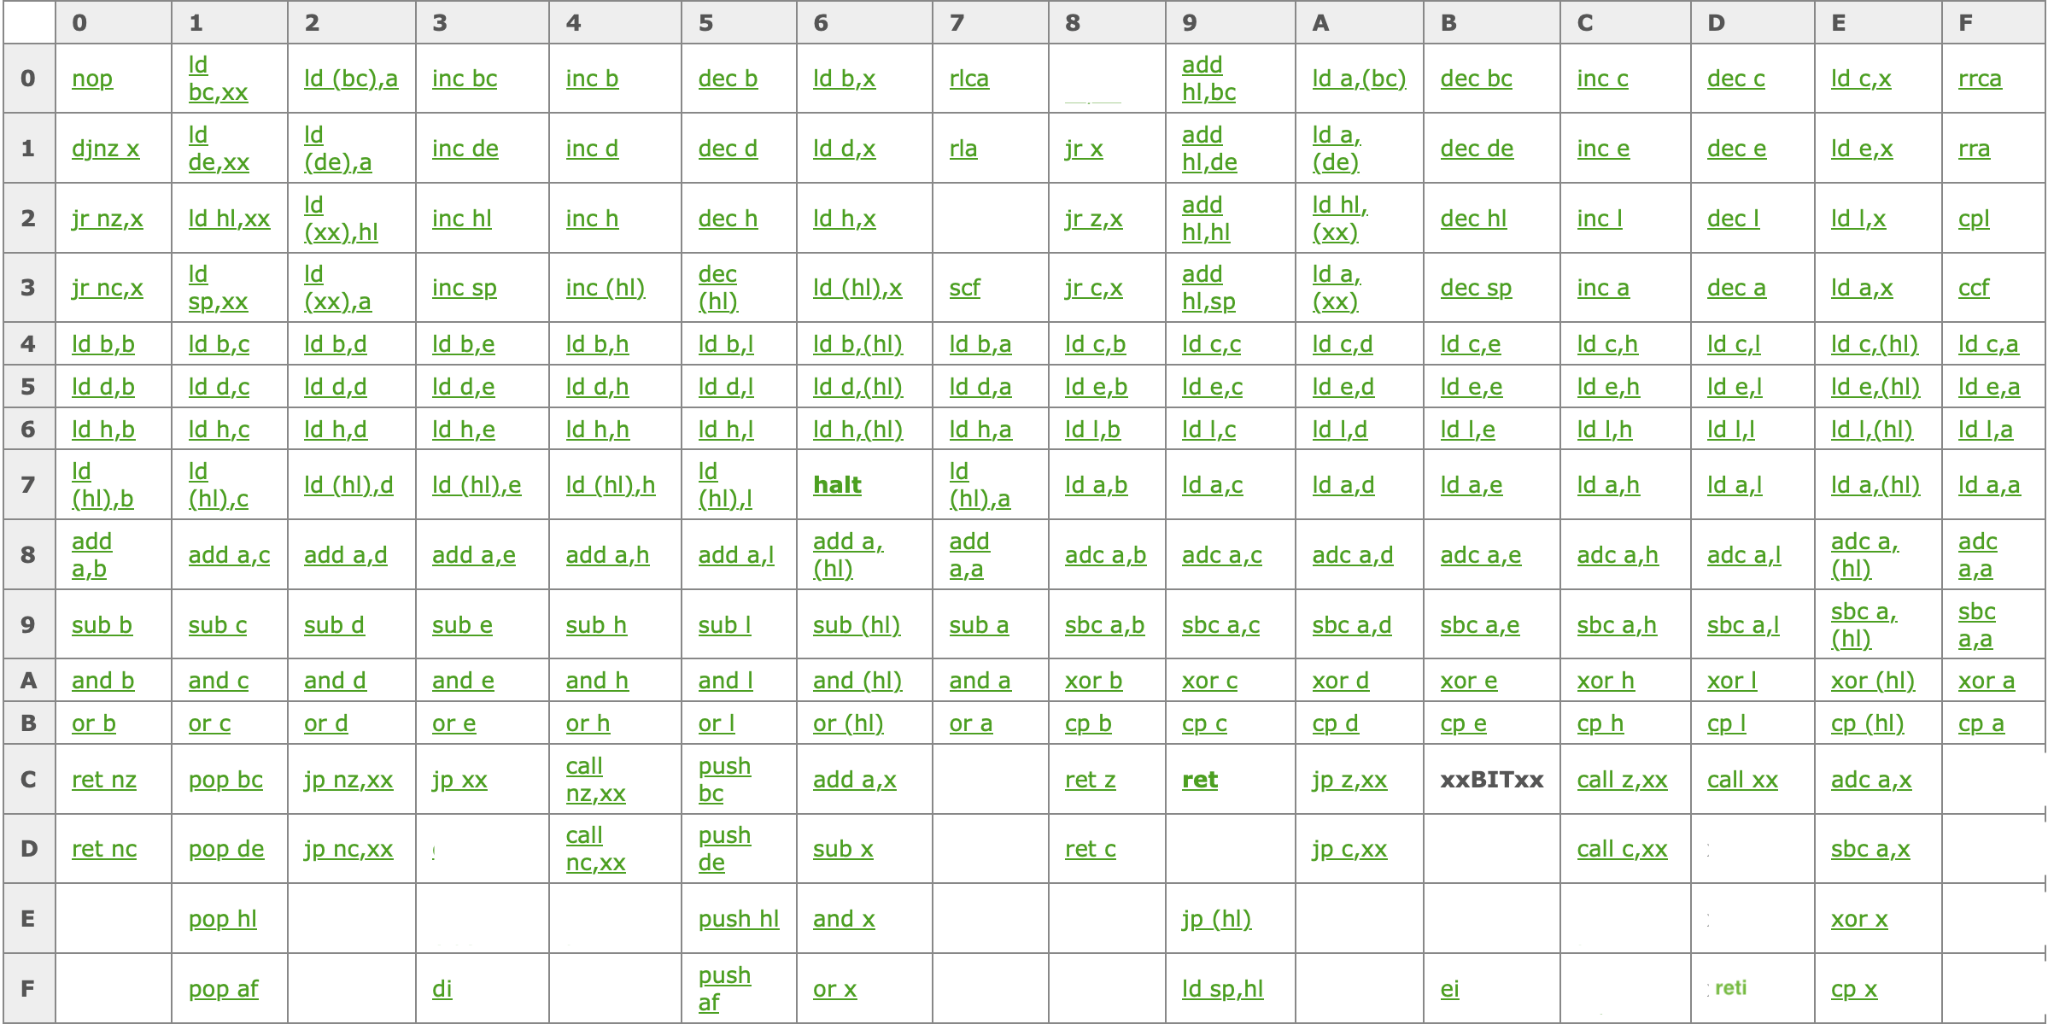
\includegraphics[width=\textwidth]{instructions.png}
		\caption{Instructions Supported}
		\label{fig:instruction_set}
	\end{minipage}
\end{figure}

\section{Memory Map}

The provided program for the Raspberry Pi Pico provides support for a simple ROM/RAM memory map in
addition to the internal memory mapped IO regions. Software wishing to use the stack needs to set
the stack pointer to a lower address such as 0x3000 (from its default value of 0xFF00) before
pushing/popping data from the stack. The memory map can be seen in Table \ref{tab:memory_map}.

\begin{table}[H]
	\centering
	\begin{tblr}{c|c|X}
		\textbf{Memory Range} & \textbf{Description} & \textbf{Usage}                                \\ \hline
		0xFFD0-0xFFD4         & Timer Access         & A register map consisting of \{enable,
		duration0, duration1, duration2, duration3\} bytes.                                          \\ \hline
		0xFFC0                & GPIO Interrupt Mask  & Setting a 1 in each bit will enable
		interrupts from that respective GPIO pin.                                                    \\ \hline
		0xFF90-0xFF97         & GPIO Pin Access      & Read/writes to these addresses will
		read/write from the GPIO pins.                                                               \\ \hline
		0xFF80-0xFF87         & GPIO Pin Control     & Setting a byte to 1 will set the
		corresponding GPIO pin to output.                                                            \\ \hline
		0x2000-0x7FFF         & RAM                  & Random access memory used for things like the
		stack and any R/W memory.                                                                    \\ \hline
		0x0000-0x2000         & ROM                  & Read only memory.                             \\ \hline
	\end{tblr}
	\caption{Memory Map}
	\label{tab:memory_map}
\end{table}

\section{Testing Schematic}

The schematic for testing the Z23 processor can be seen in Figure \ref{fig:test_schm}. The wiring
for the GPIO pins is based of the program in \verb|src/test.S| which blinks the an LED using the
GPIO0 pin. Note that IO pins 1 through 4 are skipped as they are used for the project select feature
of the NEBULA chip. IO pins 0 and 5-19 are used for the 16 address bits. IO pins 20-27 are used for the
8 data bits. IO pin 29 is the write/!read pin which is used to control whether the CPU wants to write
or read at the address. IO pin 30 is the dedicated interrupt pin. IO pins 30-37 are user
programmable GPIO pins. Note that the schematic doesn't reflect the pin out of the Raspberry Pi Pico
which is has a few ground pins which aren't shown in the schematic and should be skipped. The pinout
of the Pico can be seen in Figure \ref{fig:rpp_pinout}.\\

\begin{mdframed}[frametitle=Hardware Bug Discovered During Testing]
	During testing, it was discovered that instructions which attempt to write to memory seem
	to halt the CPU. This is not intended behavior, and is likely due to a hardware bug in the memory
	controller portion of the design. Instructions which were tested to have failed are \verb|push de|,
	\verb|push bc|, and \verb|ld (0x3000), a|. Programs which do not write to memory should work fine.
	If you are able to get memory writes to work properly, please contact me at
	\hrefblue{mailto:singh956@purdue.edu}{singh956@purdue.edu}. Thank you.
\end{mdframed}

\begin{figure}[H]
	\includegraphics[height=\textheight]{\string"Z23".pdf}
	\caption{Testing Schematic}
	\label{fig:test_schm}
\end{figure}

\begin{figure}[H]
	\includegraphics[width=\textwidth]{\string"pico_pinout".pdf}
	\caption{Raspberry Pi Pico Pinout}
	\label{fig:rpp_pinout}
\end{figure}

\section{Building and Flashing the Pico}
All code related to testing the Z23 can be found at
\hrefblue{https://github.com/devins2518/z23-bringup}{this Github repository}. While you are building
and flashing the Pico, make sure to keep the Z23 chip reset by shorting the nRST pin to ground. In
order to build the project, you must have \hrefblue{https://cmake.org}{cmake}, the
\hrefblue{https://github.com/raspberrypi/pico-sdk}{Pico SDK}, and the
\hrefblue{https://developer.arm.com/Tools\%20and\%20Software/GNU\%20Toolchain}{ARM GNU Toolchain}
installed. Additionally, the \verb|$PICO_SDK_PATH| must point to the \verb|lib/| folder in your SDK
installation. The steps to build the program for the Pico are shown below.

\begin{enumerate}
	\item \verb|git submodule update --init --recursive|
	\item \verb|pushd zasm && make zasm && popd|
	\item \verb|mkdir build && pushd build && cmake .. && make && popd|
\end{enumerate}

Once you run these commands, a .uf2 file will appear in the \verb|build/| directory. Hold the
bootsel button on the Pico as you plug it into your computer, and it should appear as a media drive
in your file explorer. Drag the .uf2 into the drive to flash the Pico. Unplug and replug the Pico
from your computer to ensure it properly starts up.

\section{Testing Files}

\subsection{\texttt{src/test.S}}
This is the default test case which will be built by default. It blinks the GPIO0 pin repeatedly by
toggling the GPIO0 control register and then waiting in spin loops.\\

\subsection{\texttt{src/blink\_gpio.S}}
This is very similar to \verb|src/test.S|, but it has a smaller toggle delay which can be seen
easier using an AD2.\\

\subsection{\texttt{src/spi\_oled.S}}
This file implements a simple SPI interface using GPIO0 as nCS, GPIO1 as SDO, and GPIO2 as SCL which
is designed to be used with the 1602A OLED display which is used in ECE 36200. It was developed
before the memory write bug was discovered, however, in theory it should work and display the letter
'a' on the screen.

\subsection{\texttt{src/z23.S}}
This file is a simple include file for any program which wishes to use the \verb|reti| instruction
to return from an interrupt. The Z23 has a nonstandard decoding of this instruction.

\subsection{\texttt{src/main.c}}
This file is the main file which is flashed onto the Pico. It essentially sits in a loop and
responds to the bus requests from the Z23 as they come in. Note that it relies on overclocking the
Pico to achieve acceptable response speeds. If you are uncomfortable with this, you can comment out
line 100 which calls \verb|set_sys_clock_khz|. After the Pico has been successfully flashed, the LED
near the bootsel button should light up.

\subsection{\texttt{src/rom.h}}
This file is generated by running the \verb|zasm| assembler on \verb|src/test.S| before building the
rest of \verb|src/main.c|. It defined an array of bytes which correspond to the ROM data generated
by the assembler.

\subsection{\texttt{layout/Z23}}
The KiCad schematic files for the Z23 testing schematic.

\end{document}
